\section{Overview of \sysname}\label{overview}

\begin{figure}
    \centering
    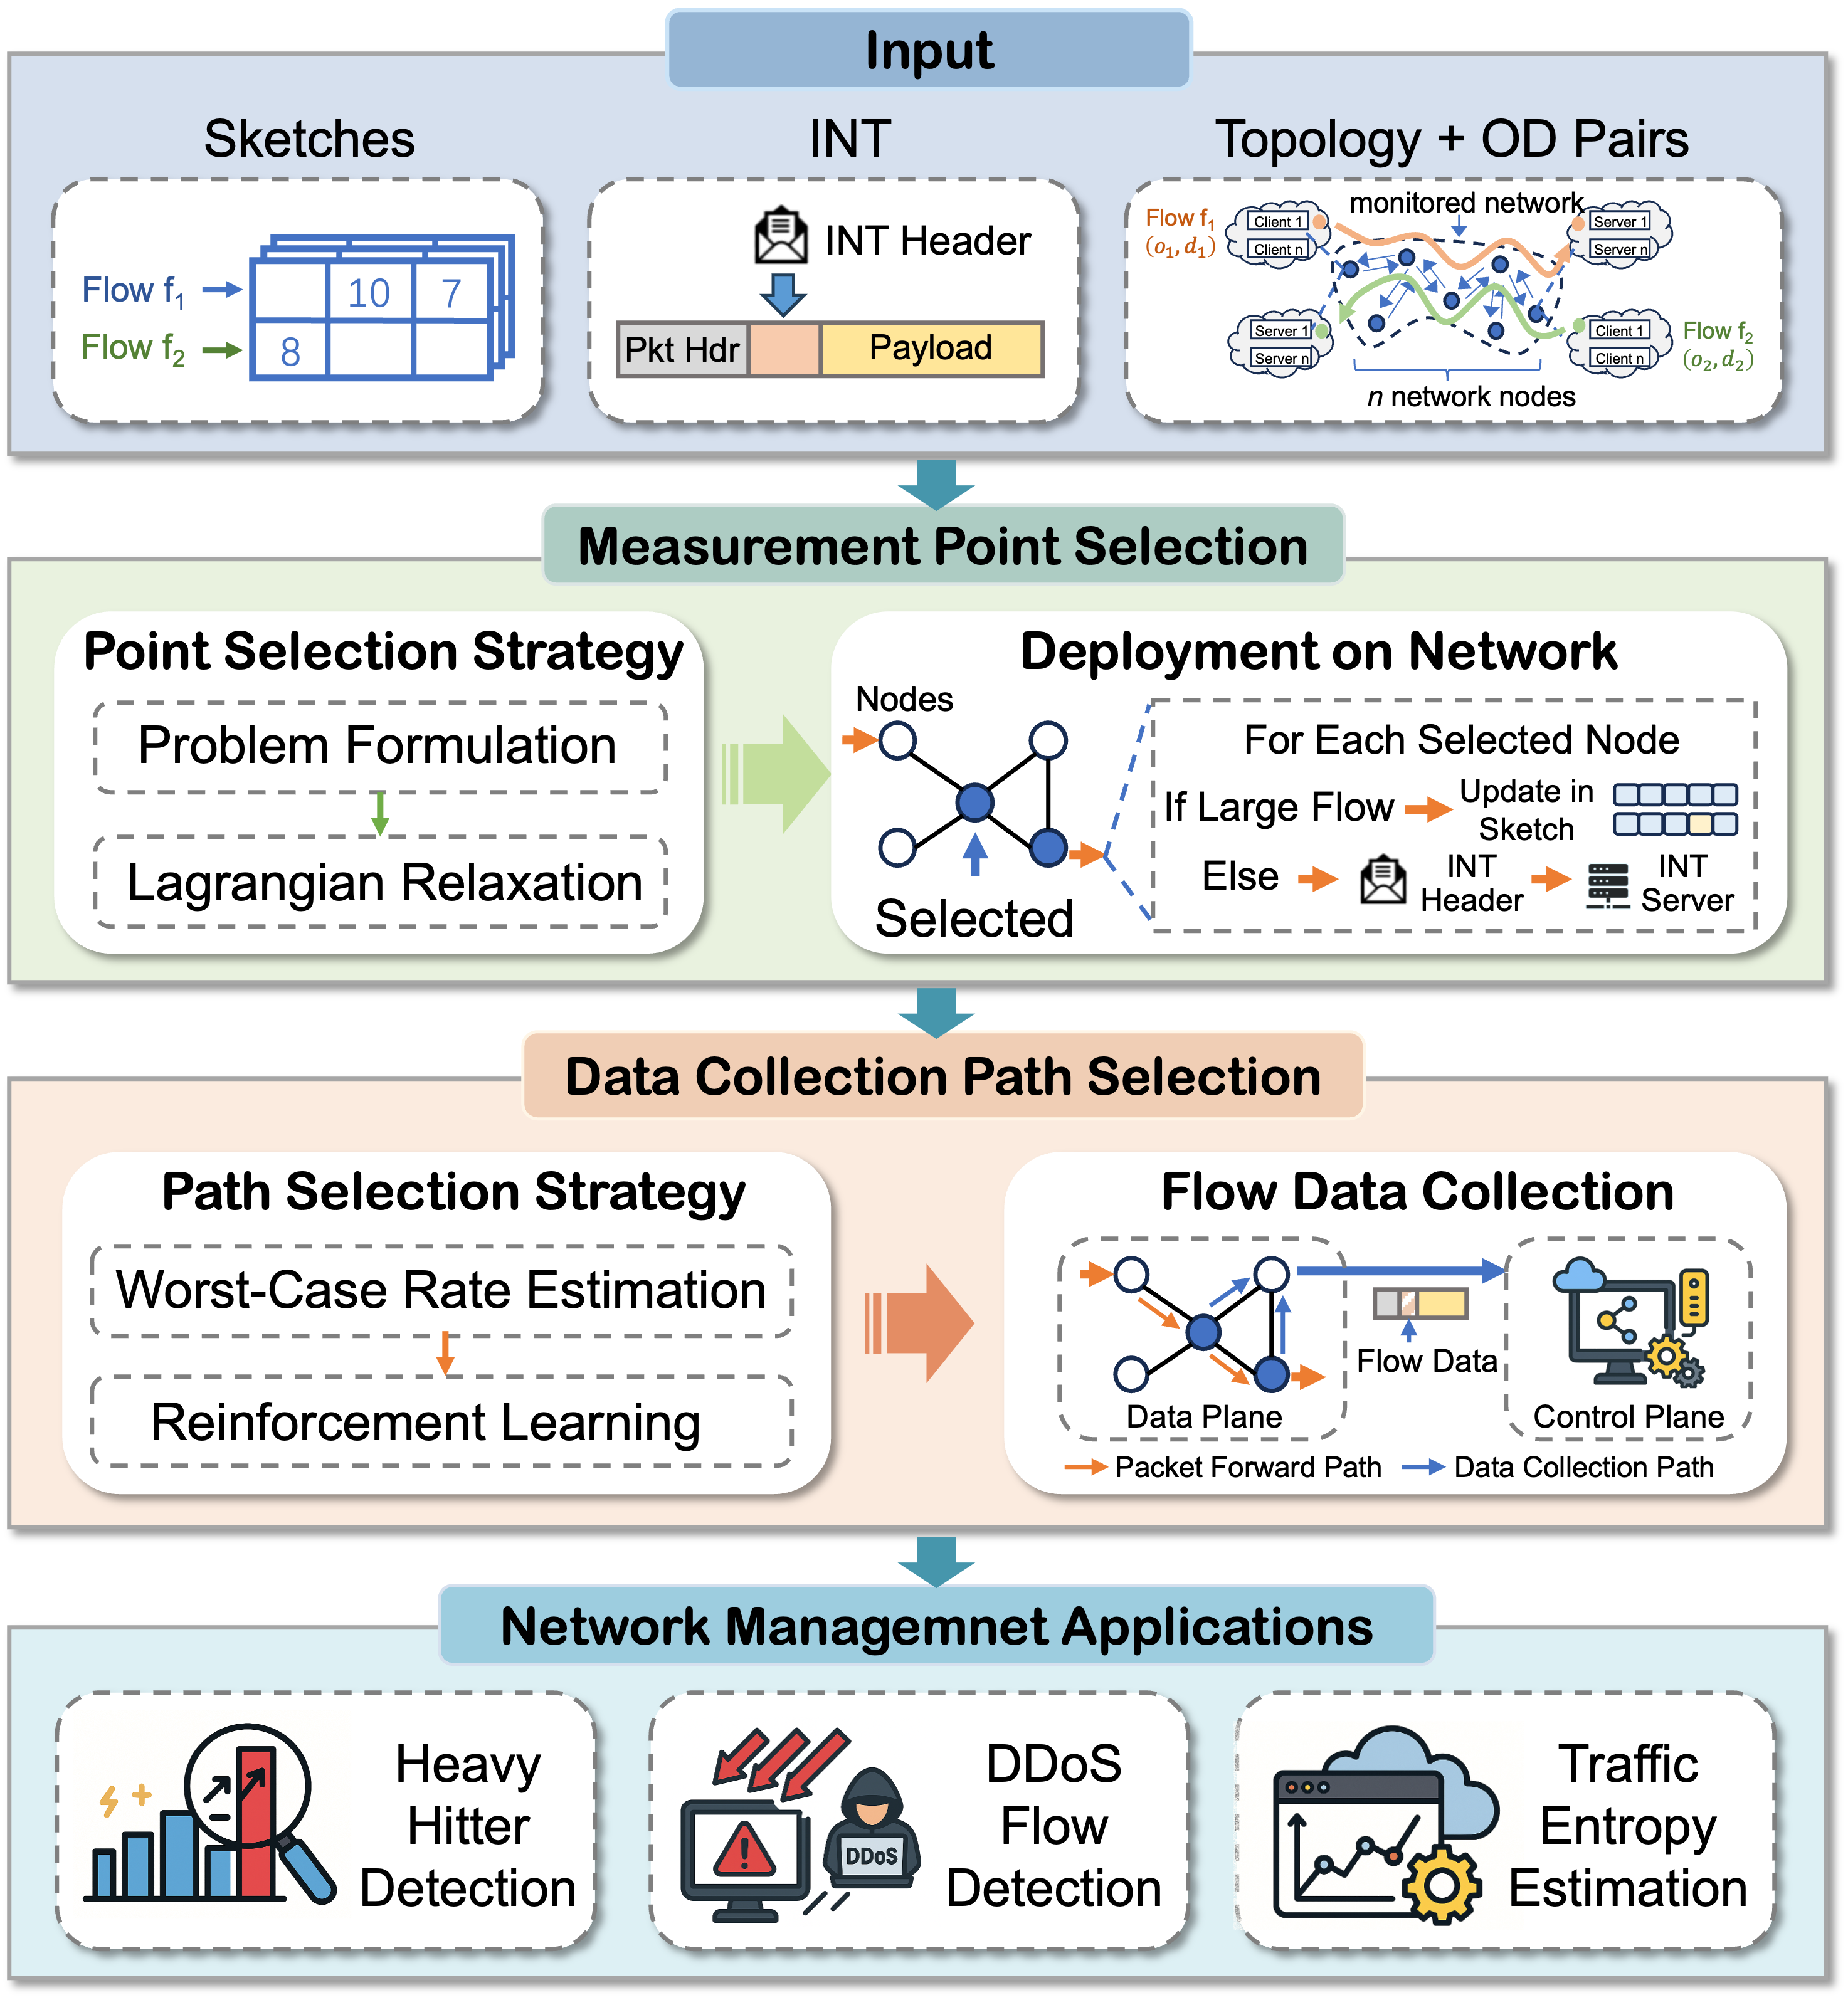
\includegraphics[width=\linewidth]{pics/overview.png}
    \caption{MonPlan overview.}
    \label{overview}
\end{figure}

\para{Goals}. We aim to achieve two goals of network measurement.

\begin{itemize}[leftmargin=*]
%
    \item \textbf{G1: High accuracy}, i.e., measuring large flows and small flows accurately (addressing \textbf{L1}, \S\ref{sketches}). 
%
    \item \textbf{G2: Resource efficiency}, i.e., avoiding high resource overheads in measurement data collection (addressing \textbf{L2}, \S\ref{int}). 
%
\end{itemize}

\para{Key idea}. According to our analysis, we observe that sketches and INT complement each other. More precisely, in Table~I, we summarize the advantages and limitations of sketches and INT: Sketches exhibit both high accuracy and resource efficiency for large flows, but they fall short for small flows; INT can provide high accuracy for both large and small flows, but they come at the cost of high resource consumption. 

In this context, we conclude the opportunities of combining sketches and INT: we can use sketches to measure large flows while using INT to measure small flows. Doing so can achieve both high accuracy and resource efficiency. In detail, traffic in modern networks is skewed \cite{roy2015inside,huang2021toward,caida,benson2010network,yang2018elastic}. So most packets originate from large flows, which are accurately and efficiently measured by sketches. For other packets from small flows, they are measured by INT, ensuring their full accuracy. Also, their number is small, limiting INT's resource consumption. Hence, both \textbf{G1} and \textbf{G2} can be achieved. 

\para{Challenges}.
However, while it is technically sound, leveraging these opportunities faces two optimization challenges.

\begin{itemize}[leftmargin=*]
%
    \item \textbf{C1: Measurement point selection with incomplete knowledge}. Traffic routing details are usually unknown in advance. As such, selecting measurement points (i.e., the switches that execute sketches and INT) is non-trivial. First, guaranteeing that every flow traverses at least one point when routing paths are unknown is challenging. This uncertainty may result in over-provisioning of measurement points, increasing deployment overheads. Second, measurement points should be close to the control plane. Otherwise, measurement data collection may suffer from high latency, delaying network management. Thus, without precise path knowledge, achieving both high coverage and low collection latency is NP-hard. 
%
%    \item \textbf{C2: General data reduction for heterogeneous measurement data}. For resource efficiency, measurement data should be minimized to save network bandwidth and control plane resources. However, such reduction faces the inherent heterogeneity between sketch data (e.g., structured counter arrays) and INT headers (e.g., unstructured hop-by-hop metadata). Specifically, reducing sketch data needs to preserve counter relationships over time, while reducing INT data should avoid modifying original per-switch information. Such differences impede the design of reducing measurement data. Without careful analysis, simply collaborating existing data reduction techniques would be ineffective and even hurt data integrity. 
%
    \item \textbf{C2: Congestion-free measurement data collection under bursts}. Measurement data from sketches and INT generates data streams that may saturate network paths connecting measurement points with the control plane. Thus, this challenge stems from the need to prevent the streams of measurement data from causing congestion during collection. For example, when thousands of incoming flows simultaneously activate INT at the switch, the resulting O(10$^2$)\,Gbps data traffic can overwhelm 100-Gbps paths in milliseconds. Thus, avoiding congestion requires complicated modeling of worst-case collection rates to prevent collisions with normal traffic. 
    %Profiling ``safe'' collection rates alone is insufficient because traffic dynamics cause rates to vary unpredictably. 
%
\end{itemize}

\para{Design}. In response, we design \sysname, a framework that co-designs sketches and INT to collectively achieve high accuracy (\textbf{G1}) and resource efficiency (\textbf{G2}). To address the above challenges, \sysname embraces two-pronged system mechanisms. 

\begin{itemize}[leftmargin=*]
%
    \item \emph{Near-optimal measurement point selection}. Given a network and a set of orientation-destination (OD) pairs, each of which represents the ingress and egress of a specific flow, \sysname chooses enough switches to place sketches and INT. It aims at maximizing the coverage of measured flows and minimizing the distance between the switches where flows are measured and the control plane where traffic statistics are collected and analyzed. Next, it formulates such an optimization as a multi-objective facility location problem and leverages Lagrangian relaxation to obtain near-optimal decisions (addressing \textbf{C1}). 
%
%    \item \emph{Resource-efficient measurement data reduction}. At runtime, sketches report their data that summaries large flow statistics to the control plane while INT keeps track of small flows. However, when all measurement data, including sketch and INT data, is collected to the control plane, their large volume can easily saturate control plane resources in a short time. In response, we analyze the characteristics of various types of measurement data. With analysis results, we design \sysname to adopt a suite of techniques, e.g., merging similar data and only sending data delta, in data collection to safely minimize data while preserving integrity (addressing \textbf{C2}). 
%
    \item \emph{Congestion-free measurement data collection}. Switches collectively report high-speed streams of measurement data to the control plane via normal network paths. Therefore, these streams may be collided with normal traffic, causing network congestion and significant data loss. To prevent congestions, \sysname automatically profiles the maximum possible rate of sending measurement data from every switch to the control plane. According to profiling results, it decides which paths to transfer data while avoiding congestion (addressing \textbf{C2}). 
%
\end{itemize}

\para{Architecture}. Figure~2 presents the architecture of \sysname, which employs a four-step workflow. 

\begin{itemize}[leftmargin=*]
%
    \item[1] Administrators submit the sketches and INT techniques they plan to use to \sysname. As a general framework, \sysname supports arbitrary types of sketches and INT techniques. 
%
    \item[2] Without precise information, \sysname solves the selection of measurement points via a Lagrangian relaxation algorithm that yields near-optimal decisions within polynomial time.
    %\sysname formulates the selection of measurement points that deploy sketches and INT to cover as many flows as possible into a multi-objective facility location problem \cite{karatas2018iterative} with coverage constraints. Thereafter, it solves this problem via a Lagrangian relaxation algorithm that yields near-optimal decisions within polynomial time. 
%
    \item[3] \sysname performs sketches and INT atop selected switches. Each flow will be first measured by sketches. If it is identified as a large flow, its data is approximately recorded by sketches. Otherwise, its data is piggybacked on its headers via INT. 
%
%    \item[4] Before emitting measurement data, i.e., periodically collecting sketch data or sending INT headers, \sysname minimizes data by using the techniques that best match each data type. 
    %\sysname minimizes data to reduce resource consumption. It first characterizes the differences between sketch data and INT data. After that, it uses corresponding data reduction techniques that best match each data type to minimize data. 
%
    \item[4] \sysname selects network paths to transfer measurement data with the goal of avoiding congestion with normal traffic. The control plane receives data, which is input to applications for subsequent network management. 
    %For each type of data emitted by each switch, \sysname estimates the worst-case rate of sending such data. According to 
%
\end{itemize}


%\para{Step-by-step example}. 

\section{Near-Optimal Measurement Point Selection}\label{selection}


\para{Overview.} The measurement point selection problem aims to select programmable switches in the network to deploy sketches and INT. It has two objectives: (1) maximizing flow coverage, i.e., measuring as many flows as possible, and (2) minimizing the distance between the control plane and switches that execute network measurement to enable timely data collection.

\begin{table}[t]
\caption{Notation of major symbols used by this paper.}
\label{tab:notation}
\centering
\resizebox{1.0\linewidth}{!}{
\small
\begin{tabular}{p{0.13\linewidth}p{0.95\linewidth}}
\toprule
\textbf{Symbol} & \textbf{Description} \\
\midrule
$G$ & Network topology with switches $V$ and links $E$ \\
$P \subseteq V$ & Programmable switches supporting sketches and INT \\
$C \subseteq V$ & Control plane nodes \\
$\mathcal{F}$ & Set of flows \\
$o_f, d_f$ & Orientation/destination of flow $f \in \mathcal{F}$ \\
$\mathcal{P}_f$ & Programmable switches on \textit{any shortest path} for flow $f$ \\
$\mathcal{F}_p$ & Flows that \textit{can be measured} at switch $p$ ($\{f \mid p \in \mathcal{P}_f\}$) \\
$\delta(p,c)$ & Distance between switch $p$ and control plane node $c$ \\
$\alpha$ & Coverage-distance tradeoff parameter ($0 \leq \alpha \leq 1$) \\
$\lambda_f$ & Lagrange multiplier for flow $f$'s coverage constraints \\
$L(\boldsymbol{\lambda})$ & Lagrangian dual function \\
$\beta_p$ & Switch penalty = $\sum_{f \in \mathcal{F}_p} \lambda_f$ \\
$\gamma_p$ & Data collection distance cost = $(1-\alpha) \min_{c \in C} \delta(p,c)$ \\
$g_f$ & Subgradient = $\sum_{p \in \mathcal{P}_f} u_p - w_f$ \\
$T$ & Iteration count in subgradient optimization \\
$\pi_\theta$ & Trained RL policy network \\
$\mathcal{P}_{p,c}$ & Selected network path from switch $p$ to control plane node $c$ \\
$\pi_{p,c}$ & Fraction of measurement data traffic from $p$ to $c$ \\
$q_e^t$ & Queue depth (bytes) on link $e$ at time $t$ \\
$\Gamma_p^{\text{total}}$ & Worst-case measurement data rate (bps) at switch $p$ \\
$\Gamma_e^{\text{data}}$ & Normal data plane traffic rate (bps) on link $e$ \\
$\tau_e$ & Safety threshold for congestion avoidance on link $e$ \\
$s_t$ & State vector at time $t$ for RL policy \\
$x_p$ & 0-1 variable = 1 if sketch deployed at switch $p$ \\
$y_p$ & 0-1 variable = 1 if INT deployed at switch $p$ \\
$u_p$ & 0-1 variable = 1 if switch $p$ is selected ($x_p=1 \lor y_p=1$) \\
$z_{p,c}$ & 0-1 variable = 1 if data emitted from $p$ to control plane node $c$ \\
$w_f$ & 0-1 variable = 1 if flow $f$ is covered (i.e., measured) \\
\bottomrule
\end{tabular}}
\end{table}

% \begin{table}[t]
% \caption{Notation of major symbols used by this paper.}
% \label{notation}
% \newcommand{\tabincell}[2]{\begin{tabular}{@{}#1@{}}#2\end{tabular}}
% \centering
% \resizebox{1.0\linewidth}{!}{
% \small
% \begin{tabular}{p{0.13\linewidth}p{0.95\linewidth}}
% \toprule
% \textbf{Symbol} & \textbf{Description} \\
% \midrule
% $G$ & Network $G = (V, E)$: $V$ contains switches; $E$ contains links \\
% $P \subseteq V$ & Programmable switches that enable sketches and INT \\
% $C \subseteq V$ & Control plane nodes \\
% $\mathcal{F}$ & Set of flows \\
% $o_f, d_f$ & Orientation/destination of flow $f \in \mathcal{F}$ \\
% $\mathcal{P}_f$ & Programmable switches on shortest paths for flow $f$ \\
% $\delta(p,c)$ & Distance between switch $p$ and control node $c$ \\
% $\alpha$ & Coverage-distance tradeoff parameter ($0 \leq \alpha \leq 1$) \\
% $x_p$ & 0-1 variable indicating sketch deployment at switch $p$ \\
% $y_p$ & 0-1 variable indicating INT deployment at switch $p$ \\
% $u_p$ & 0-1 variable indicating measurement activation at switch $p$ \\
% $z_{p,c}$ & 0-1 variable indicating data routing from $p$ to control node $c$ \\
% $w_f$ & 0-1 variable indicating flow coverage \\
% \bottomrule
% \end{tabular}}
% \end{table}

\para{Input.} The input comprises:
(1) the network $G = (V, E)$;
(2) programmable switches $P \subseteq V$ supporting sketches and INT;
(3) control plane nodes $C \subseteq V$;
(4) a set $\mathcal{F}$ of flows, where each flow $f \in \mathcal{F}$ only indicates an OD pair $(o_f, d_f)$ \cite{liu2016one,anup2022hetero}, where $o_f$ and $d_f$ are the ingress and egress of $f$, respectively; 
(5) for each flow $f$, the set $\mathcal{P}_f \subseteq P$ of switches on \emph{any shortest path} between $o_f$ and $d_f$;
and (6) the distance metric $\delta: V \times C \to \mathbb{R}^+$ (e.g., hop count between meaurement points and control plane).

\para{Output.} The output comprises:
(1) $x_p \in \{0,1\}$ $\forall p \in P$: $x_p=1$ if sketch deployed at switch $p$;
(2) $y_p \in \{0,1\}$ $\forall p \in P$: $y_p=1$ if INT deployed at switch $p$;
(3) $u_p \in \{0,1\}$ $\forall p \in P$: $u_p=1$ if switch $p$ is selected ($x_p =1 \lor y_p=1$);
(4) $z_{p,c} \in \{0,1\}$ $\forall p \in P, c \in C$: $z_{p,c}=1$ if data from $p$ sent to control node $c$;
and (5) $w_f \in \{0,1\}$ $\forall f \in \mathcal{F}$: $w_f=1$ if flow $f$ is covered.

\para{Objective.} The objective refers to:
\begin{equation}
\min\ -\alpha \sum_{f \in \mathcal{F}} w_f + (1-\alpha) \sum_{\substack{p \in P \\ c \in C}} z_{p,c} \cdot \delta(p, c)
\label{eq:objective}
\end{equation}
where the user-configurable parameter $\alpha \in [0,1]$ balances the objective of maximizing coverage and that of minimizing the distances between selected switches and control plane nodes. 

\para{Constraints.} The problem has the following major constraints: Eq.2-4 bound the number of selected switches; Eq.5 presents that when a flow $f$ is covered, at least one switch on the shortest paths that connect the OD pair of $f$ should be selected; Eq.6 shows that each selected switch should send data to a control plane node; and Eq.7 limits decision variables. 

\vspace{-7pt}
{\footnotesize
\begin{align}
\text{Selected switch number: } &u_p \geq x_p \quad \forall p \in P \\
&u_p \geq y_p \quad \forall p \in P \\
&u_p \leq x_p + y_p \quad \forall p \in P \\
\text{Coverage: } &w_f \leq \sum_{p \in \mathcal{P}_f} u_p \quad \forall f \in \mathcal{F} \\
\text{Data collection: } &\sum_{c \in C} z_{p,c} = u_p \quad \forall p \in P \\
\text{0-1 decisions: } &x_p, y_p, u_p, w_f, z_{p,c} \in \{0,1\}
\end{align}}

There also exist other objectives, e.g., maximizing the number of covered switches or the number of covered links. While our focus is flow coverage, supporting other objectives is still simple, i.e., replacing Eq.1 with user-specified objectives. 

\para{Hardness}. This measurement point selection problem is NP-hard. First, according to its dual combinatorial structures, this problem reduces to the set cover problem: each programmable switch $p \in P$ corresponds to the set $S_p = \{ f \in \mathcal{F} \mid p \in \mathcal{P}_f \}$ covering the flows possibly traversing $p$. This step establishes a set system with the universe $U = \mathcal{F}$ and collection $\mathcal{S} = \{ S_p \}$, where maximizing coverage $\sum w_f$ equals minimizing uncovered flows (i.e., a standard NP-hard set cover problem). Second, the objective of minimizing distances, i.e., $\sum z_{p,c} \delta(p,c)$, forms an uncapacitated facility location subproblem, in which selected switches, i.e., $u_p=1$, are facilities, control plane nodes in $C$ are clients, and $\delta(p,c)$ are assignment costs. 

To sum up, the joint objective in Eq.1 forms a multi-objective set cover with facility location costs. In particular, $\alpha$ modulates between flow coverage and resource efficiency: when $\alpha=1$, the problem is an NP-hard set cover problem; when $\alpha=0$, the problem is an NP-hard facility location problem.  


\para{Solving}. Given the NP hardness, directly solving the problem using commercial MIP solvers such as Gurobi \cite{gurobi} and CPLEX \cite{cplex} inevitably suffers from excessively long execution time or fails to find possible solutions. In response, \sysname employs Lagrangian relaxation as follows.

We relax the coverage constraints using Lagrange multipliers \(\lambda_f \geq 0\). The Lagrangian is:

\vspace{-10pt}
{\footnotesize
\begin{align}
L(\boldsymbol{\lambda}) = &\min_{\mathbf{u},\mathbf{w},\mathbf{z}} \left[ 
-\alpha \sum_{f} w_f + (1-\alpha) \sum_{p,c} z_{p,c} \delta(p,c) \right. \nonumber \\ &\left. + \sum_{f} \lambda_f \left( \sum_{p \in \mathcal{P}_f} u_p - w_f \right)
\right] 
= \min_{\mathbf{u},\mathbf{w},\mathbf{z}} \left[ 
\underbrace{\sum_{p} u_p \left( \sum_{f: p \in \mathcal{P}_f} \lambda_f \right)}_{\text{Switch penalty}} \right. \nonumber \\ &+ \left.
\underbrace{\sum_{f} w_f (-\alpha - \lambda_f)}_{\text{Coverage reward}} +
\underbrace{(1-\alpha) \sum_{p,c} z_{p,c} \delta(p,c)}_{\text{Data collection distance cost}}
\right]
\end{align}}
\vspace{-7pt}

\noindent where $\lambda_f$ is the Lagrange multiplier for flow $f$ and quantifies the penalty weight for not covering $f$. The switch penalty refers to the penalty for selecting a switch. It represents that selecting a switch needs to pay the penalty of covering all its measurable flows. Therefore, it transforms the original coverage constraints into switch selection penalties that balance against the reward of covering flows and the distance cost of transferring data from selected switches to the control plane. 

In this context, the dual of the Lagrangian relaxation is:
\begin{align}
\max_{\lambda_f \geq 0} L(\boldsymbol{\lambda}) 
\end{align}
subject to primal constraints in Eq.2-Eq.7. 
%The solution is attained via subgradient ascent: $\lambda_f^{(t+1)} = \max\left(0, \lambda_f^{(t)} + \frac{1}{\sqrt{t}} \left( \sum_{p \in \mathcal{P}_f} u_p - w_f \right)\right)$.

\begin{algorithm}[t]
\caption{Solve \( L(\boldsymbol{\lambda}) \)}
\label{alg:solve-lagrangian}
\begin{algorithmic}[1]
\footnotesize
\Require \(\boldsymbol{\lambda}\), \(G\), \(\mathcal{F}\), \(P\), \(C\), \(\delta\), \(\alpha\) (See Table~I)
\Ensure \(L(\boldsymbol{\lambda})\), primal variables
\State Initialize \(u_p = 0\), \(w_f = 0\) \(\forall p \in P, f \in \mathcal{F}\)
\For{each switch \(p \in P\)}
  \State Compute \(\beta_p = \sum_{f: p \in \mathcal{P}_f} \lambda_f\) \Comment{{\color{aogreen}Aggregate flow penalties}}
  \State Compute \(\gamma_p = (1-\alpha) \min_{c \in C} \delta(p, c)\) \Comment{{\color{aogreen}Minimize distance costs}}
  \If{$\beta_p > \gamma_p$} \Comment{{\color{aogreen}Penalties overwhelm benefits}}
    \State Set \(u_p = 1\)
    \State Assign \(z_{p,c^*} = 1\) for \(c^* = \arg\min_c \delta(p,c)\)
  \EndIf
\EndFor
\For{each flow \(f \in \mathcal{F}\)}
  \If{$\exists p \in \mathcal{P}_f : u_p = 1$} 
    \State Set \(w_f = 1\) 
  \EndIf
\EndFor
\State \Return \(L(\boldsymbol{\lambda}) = \sum_p u_p (\beta_p + \gamma_p) + \sum_f w_f (-\alpha - \lambda_f)\)
\end{algorithmic}
\end{algorithm}

\begin{algorithm}[t]
\caption{Subgradient Optimization for Dual Problem}
\label{alg:subgradient}
\begin{algorithmic}[1]
\footnotesize
\Require Max iterations \(T\), \(\epsilon = 10^{-6}\)
\Ensure \(\max_t L(\boldsymbol{\lambda}^{(t)})\)
\State Initialize \(\lambda_f^{(0)} = 0.5\), \(\forall f \in \mathcal{F}\), \(t = 0\)
\State \(L_{\text{best}} \leftarrow -\infty\), \(\boldsymbol{\lambda}_{\text{best}} \leftarrow \boldsymbol{\lambda}^{(0)}\)
\While{\(t < T\)}
  \State Solve \(L(\boldsymbol{\lambda}^{(t)})\) using Algorithm \ref{alg:solve-lagrangian}
  \State Compute subgradient $g_f^{(t)} = \sum_{p \in \mathcal{P}_f} u_p^* - w_f^*$ $\forall f \in \mathcal{F}$
  \State Compute gradient norm \(\|g^{(t)}\| = \sqrt{\sum_f (g_f^{(t)})^2}\)
  \State Compute step size \(\theta_t = \frac{1}{\sqrt{t+1}} \cdot \frac{|L(\boldsymbol{\lambda}^{(t)})|}{\max(\|g^{(t)}\|^2,\ \epsilon)}\)
  \For{each flow \(f \in \mathcal{F}\)}
    \State \(\lambda_f^{(t+1)} = \max\left(0, \min\left(2, \lambda_f^{(t)} + \theta_t g_f^{(t)}\right)\right)\) 
  \EndFor
  \If{\(L(\boldsymbol{\lambda}^{(t)}) > L_{\text{best}}\)}
    \State \(L_{\text{best}} \leftarrow L(\boldsymbol{\lambda}^{(t)})\)
    \State \(\boldsymbol{\lambda}_{\text{best}} \leftarrow \boldsymbol{\lambda}^{(t)}\)
  \EndIf
  \State $t \leftarrow t + 1$
\EndWhile
\State \Return \(L_{\text{best}}, \boldsymbol{\lambda}_{\text{best}}\)
\end{algorithmic}
\end{algorithm}

According to the above relaxation, \sysname uses a master-slave algorithm to solve the problem: Algorithm~2 is the master that controls the optimization while Algorithm~1 is the slave that is invoked in each iteration to solve the Lagrangian subproblem. Specifically, Algorithm~2 iteratively tunes Lagrange multipliers $\boldsymbol{\lambda}$ to maximize the dual function. In each iteration $t$, it (1) inputs $\boldsymbol{\lambda}^{(t)}$ to Algorithm~1, (2) receives primal variables $u_p, w_f, z_{p,c}$ and the dual bound $L(\boldsymbol{\lambda})$, (3) computes the normalized subgradient $g_f^{(t)}$, and updates $\boldsymbol{\lambda}^{(t+1)}$ while recording the best solution.

In the step (1) of each iteration in Algorithm~2, Algorithm~1 computes the optimal deployments for given $\boldsymbol{\lambda}$: for each switch $p$, it calculates the flow penalty $\beta_p$ and collection cost $\gamma_p$. If $\beta_p > \gamma_p$, it selects $p$ to activate measurement, i.e., $u_p=1$, and assigns $p$ to the nearest control plane node, i.e., $z_{p,c^*}=1$. Next, for each flow $f$, it marks $w_f=1$ if there exists at least one selected switch on the flow's path (i.e., $\exists p \in \mathcal{P}_f: u_p=1$).

% \begin{figure}
%     \centering
%     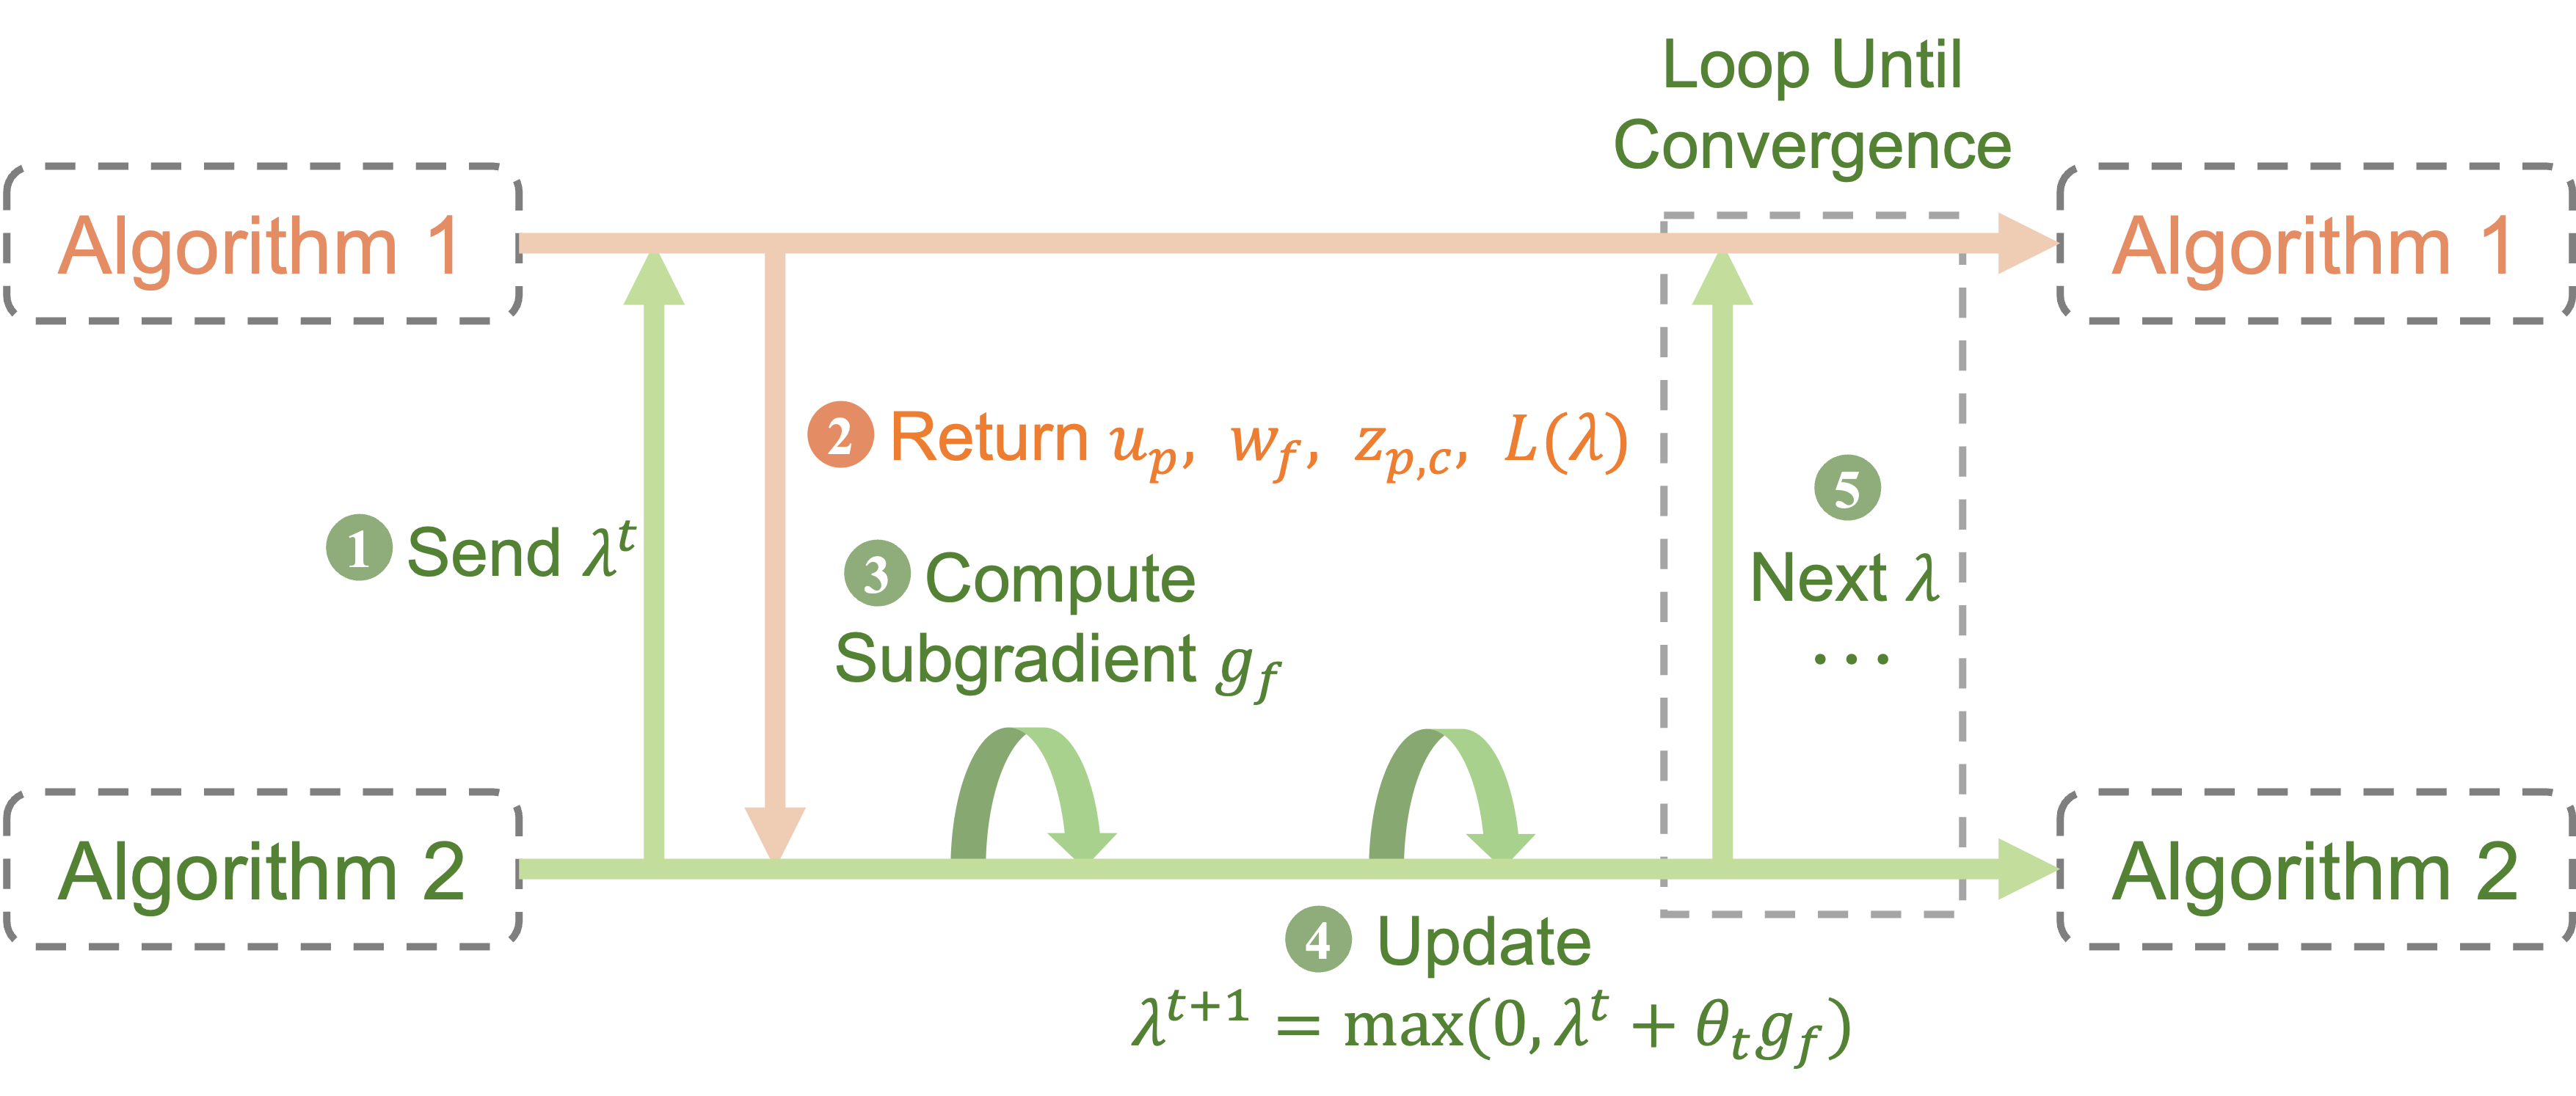
\includegraphics[width=\linewidth]{pics/lglr.png}
%     \caption{Lagrange relaxation of MonPlan.}
%     \label{lglr}
% \end{figure}

\begin{theorem}[Weak Duality]
The optimal dual value \(d^* = \max_{\boldsymbol{\lambda}} L(\boldsymbol{\lambda})\) is a lower bound on the primal optimal value \(p^*\).
% \[
% d^* \leq p^*
% \]
\end{theorem}

\begin{proof}
For any feasible primal solution \((\mathbf{u},\mathbf{w},\mathbf{z})\) and \(\boldsymbol{\lambda} \geq 0\):
{\footnotesize
\[
\begin{aligned}
L(\boldsymbol{\lambda}) &\leq -\alpha \sum_f w_f + (1-\alpha) \sum_{p,c} z_{p,c} \delta(p,c) \\
&+ \sum_f \lambda_f \left( \sum_{p \in \mathcal{P}_f} u_p - w_f \right) \\
&\leq -\alpha \sum_f w_f + (1-\alpha) \sum_{p,c} z_{p,c} \delta(p,c) \\
&= p_{\text{obj}} \quad \text{(since } \sum_{p \in \mathcal{P}_f} u_p - w_f \geq 0 \text{ by Eq.5)}
\end{aligned}
\]
}

\noindent where $p_{\text{obj}}$ is the primal objective value for a feasible solution in the measurement point selection problem. Thus, \(d^* \leq p^*\).
\end{proof}

\begin{theorem}[Optimality Gap]
Let \((\mathbf{u}^*,\mathbf{w}^*,\mathbf{z}^*)\) be the primal optimal solution. The optimality gap satisfies:
\[
p^* - d^* \leq \sum_{f \in \mathcal{F}} \lambda_f^* \left( \sum_{p \in \mathcal{P}_f} u_p^* - w_f^* \right)
\]
where \(\boldsymbol{\lambda}^*\) are the optimal dual multipliers.
\end{theorem}

\begin{proof}
From complementary slackness:
{\footnotesize
\[
\begin{aligned}
p^* - d^* &= \left[ -\alpha \sum_f w_f^* + (1-\alpha) \sum_{p,c} z_{p,c}^* \delta(p,c) \right] - L(\boldsymbol{\lambda}^*) \\
&= \sum_f \lambda_f^* \left( w_f^* - \sum_{p \in \mathcal{P}_f} u_p^* \right) \\
&\leq 0 \quad \text{(because } w_f^* \leq \sum_{p \in \mathcal{P}_f} u_p^* \text{ and } \lambda_f^* \geq 0\text{)}
\end{aligned}
\]
}

\noindent The gap equals the sum of violated coverage constraints scaled by \(\lambda_f^*\).
\end{proof}

% \begin{theorem}[Time Complexity]
% Given a network $G = (V, E)$, programmable switches in $P \subseteq V$, control plane nodes in $C \subseteq V$, flows in $\mathcal{F}$, and flow-switch incidence sets $\{\mathcal{P}_f\}$, the time complexity of Algorithms 1-2 is $O(T \cdot |P| \cdot (d_{\max} + |C|))$, where $T$ is the iteration count, $d_{\max} = \max_{p \in P} |\{f : p \in \mathcal{P}_f\}|$, and $|C|$ is the number of control plane nodes.
% \end{theorem}

% \begin{proof}
% The complexity is contributed by all the $T$ iterations of Algorithm 2, each of which invokes Algorithm 1. For Algorithm 1, it invokes: (1) for each $p \in P$, it computes $\beta_p = \sum_{f: p \in \mathcal{P}_f} \lambda_f$ in $O(d_p)$ time, where $d_p = |\{f : p \in \mathcal{P}_f\}| \leq d_{\max}$, (2) for each $p \in P$, it computes $\gamma_p = (1-\alpha) \min_{c \in C} \delta(p,c)$ in $O(|C|)$ time, (3) for each $p \in P$, it sets decision variables in $O(1)$ time. Thus, the time complexity of Algorithm 1 is $O(|P| \cdot (d_{\max} + |C|))$. For Algorithm 2, each iteration invokes: (1) $O(|P| \cdot (d_{\max} + |C|))$ Algorithm 1, (2) computing subgradient $g_f = \sum_{p \in \mathcal{P}_f} u_p$ for all $f \in \mathcal{F}$ in $O\left(\sum_f |\mathcal{P}_f|\right) = O(|P| \cdot d_{\max})$ time, and (3) updating multipliers in $O(|\mathcal{F}|) \subseteq O(|P| \cdot d_{\max})$ time. Thus, Algorithm~2 has $T$ iterations, yielding $O(T \cdot |P| \cdot (d_{\max} + |C|))$.
% \end{proof}

% \begin{theorem}[Algorithm~1 Complexity]
% The time complexity of Algorithm~1 is $\mathcal{O}(|P| \cdot (d_{\max} + |C|))$, where $|P|$ is the number of switches, $d_{\max} = \max_{p \in P} |\{f : p \in \mathcal{P}_f\}|$, and $|C|$ is the number of control plane nodes.
% \end{theorem}

% \begin{proof}
% For each switch $p$, Algorithm 1 performs (1) $\beta_p$ computation (line~3), which complexity is $\mathcal{O}(d_p)$ ($d_p$ counts how many flows can potentially be measured by $p$), (2) $\gamma_p$ computation (line~4), which complexity is $\mathcal{O}(|C|)$, and (3) making decisions (lines~5-7), which complexity is $\mathcal{O}(1)$. To sum up, the 

% Summing over $p$: $\sum_p \mathcal{O}(d_p) = \mathcal{O}(|P| \cdot d_{\max})$. Adding coverage marking $\mathcal{O}(|\mathcal{F}|)$ and noting $|\mathcal{F}| \leq |P| \cdot d_{\max}$, total complexity is $\mathcal{O}(|P| \cdot (d_{\max} + |C|))$.
% \end{proof}

% \begin{theorem}[Algorithm 2 Complexity]
% The time complexity for $T$ iterations of Algorithm 2 is $\mathcal{O}(T \cdot |P| \cdot (d_{\max} + |C|))$.
% \end{theorem}

% \begin{proof}
% Each iteration involves:
% \begin{itemize}
%   \item Algorithm 1 call: $\mathcal{O}(|P| \cdot (d_{\max} + |C|))$
%   \item Subgradient computation: $\mathcal{O}(|\mathcal{F}| \cdot s_{\max}) \subseteq \mathcal{O}(|P| \cdot d_{\max})$ (since $\sum_f |\mathcal{P}_f| = \sum_p d_p$)
%   \item Multiplier update: $\mathcal{O}(|\mathcal{F}|)$
% \end{itemize}
% Total per iteration: $\mathcal{O}(|P| \cdot (d_{\max} + |C|))$. For $T$ iterations: $\mathcal{O}(T \cdot |P| \cdot (d_{\max} + |C|))$.
% \end{proof}

% to the coverage constraints $w_f \leq \sum_{p \in \mathcal{P}_f} u_p$ by introducing multipliers $\lambda_f \geq 0$. The Lagrangian dual function is:

% {\footnotesize
% \begin{equation}
% L(\boldsymbol{\lambda}) = \min \left[ 
% \sum_{p} u_p \left( \sum_{f: p \in \mathcal{P}_f} \lambda_f \right) + \sum_{f} w_f (-\alpha - \lambda_f) + (1-\alpha) \sum_{p,c} z_{p,c} \delta(p,c)
% \right],
% \end{equation}}

% \noindent subject to switch usage (Eq. \ref{eq:u_x}--\ref{eq:u_sum}), control assignment (Eq. \ref{eq:control}), and binarity constraints. This decouples into: (1) Switch activation: for each $p$, set $u_p = 1$ if $\sum_{f: p \in \mathcal{P}_f} \lambda_f + (1-\alpha) \min_c \delta(p,c) < 0$, and assign $z_{p,c^*}=1$ for nearest $c^*$; (2) Coverage: set $w_f=1$ $\forall f$ (since $-\alpha - \lambda_f < 0$). We maximize $L(\boldsymbol{\lambda})$ via subgradient optimization: initialize $\lambda_f=0$; update $\lambda_f^{(t+1)} = \max\left(0, \lambda_f^{(t)} + \frac{1}{\sqrt{t}} \left( \sum_{p \in \mathcal{P}_f} u_p^* - w_f^* \right)\right)$ for $T$ iterations.

% \textbf{Optimality Analysis.}
% By weak duality, $d^* = \max_{\boldsymbol{\lambda}} L(\boldsymbol{\lambda}) \leq p^*$ for all $\boldsymbol{\lambda} \geq 0$, as $L(\boldsymbol{\lambda}) \leq$ primal objective when constraints hold. The gap $p^* - d^*$ is bounded by $\sum_f \lambda_f^* \left( \sum_{p \in \mathcal{P}_f} u_p^* - w_f^* \right)$, vanishing when coverage constraints are tight. Primal recovery achieves $\epsilon$-optimal solutions with $p_{\text{found}} \leq p^* + \epsilon$ via switch activation heuristics.


\section{Loss-Free Measurement Data Collection}\label{collection}

\para{Overview}. After making decisions on which switches to measure traffic, \sysname determines which network paths to safely transfer measurement data from switches to control plane nodes without incurring congestion. It executes a two-step workflow. First, it estimates the worst-case sending rate of sketch data and INT data in each switch. Second, according to its estimates, it picks paths to transfer data without congestion.

\para{Estimating worst-case sending rates}. \sysname models both sketch and INT data. For sketch data, the worst-case sending rate $\gamma_k^{\text{sketch}}$ for sketch $k$ is determined by:

\vspace{-4pt}
\begin{align}
\gamma_k^{\text{sketch}} = \frac{S_k}{T_k}
\end{align}

\noindent where $S_k$ and $T_k$ refer to the sketch size in bytes and the collection window in seconds, respectively. This equation denotes that the data recorded in sketch counter arrays are periodically flushed to the control plane at the end of each window, e.g., for the sketch with 10\,MB memory, a measurement window of 1\,ms corresponds to a $\gamma_k^{\text{sketch}}=\frac{10^{6}\,\text{bytes}}{10^{-3}\,\text{s}}=8\,\text{Gbps}$.  

For INT data, the worst-case rate $\gamma_p^{\text{INT}}$ at switch $p$ is:

\vspace{-4pt}
\begin{align}
\gamma_p^{\text{INT}} = \left( \frac{C_p \times \phi}{\mu} \right)\times B_{\text{INT}} 
\end{align}

\noindent where $C_p$ refers to the bandwidth capacity of each link while $\phi$ is the maximum possible fraction of link bandwidth that can be consumed by small flows. $\phi$ can be obtained by analyzing historical traffic data \cite{roy2015inside}. $C_p\times \phi$ denotes the maximum possible byte rate contributed by small flows on a link. Moreover, since INT overheads are per-packet, \sysname converts the byte rate of $C_p\times \phi$ to the packet rate to estimate INT overheads, where $\mu$ denotes the average packet size in small flows. As such, the maximum packet rate of small flows becomes $\frac{C_p \times \phi}{\mu}$. So Eq.10 estimates the bandwidth overheads consumed by INT headers per second, where $B_{\text{INT}}$ is the size of INT headers per packet. 

To sum up, the maximum possible rate of sending measurement data at switch $p$ is estimated as

\vspace{-4pt}
\begin{align}
\Gamma_p^{\text{total}} = \sum_{k \in \mathcal{K}_p} \gamma_k^{\text{sketch}} + \gamma_p^{\text{INT}}
\end{align}

\noindent where $\mathcal{K}_p$ is the set of sketches at $p$. 

%$\Gamma_p^{\text{total}}$ represents the peak load at $p$.

\para{Reinforcement learning (RL) for dynamic path selection}. Given the worst-case estimates in $\{\Gamma_p^{\text{total}}\}$, \sysname formulates dynamic path selection based on a constrained Markov decision process (CMDP) to avoid saturating network paths, i.e.

\vspace{-4pt}
\begin{align}
\min_{\pi}  & \quad \mathbb{E}\left[\sum_{t=0}^T \sum_{e \in E} q_e^t \right] \\
\text{s.t.} & \quad \sum_{c \in C} \pi_{p,c} = 1 \quad \forall p \in P  \\
            & \quad \Gamma_e^{\text{meas}} \leq \tau_e C_e - \Gamma_e^{\text{data}} \quad \forall e \in E 
\end{align}

\noindent where $q_e^t$ represents the queue depth in bytes on link $e$ at time $t$; $\pi_{p,c}$ is the fraction of measurement data streams from switch $p$ to control plane node $c$; $\Gamma_e^{\text{meas}}$ quantifies the measurement data streams on link $e$, i.e. 

\vspace{-4pt}
\begin{align}
    \Gamma_e^{\text{meas}} = \sum_{p} \sum_{c} \pi_{p,c} \cdot \Gamma_p^{\text{total}} \cdot \mathbb{I}_{e \in \mathcal{P}_{p,c}}
\end{align}

\noindent where $\mathbb{I}_{e \in \mathcal{P}_{p,c}}=1$ if link $e$ belongs to path $\mathcal{P}_{p,c}$; $\Gamma_e^{\text{data}}$ quantifies data plane traffic on $e$; and $\tau_e$ represents the safety threshold that avoids congestion (e.g., 0.8 of the link capacity).

Here, the inputs include $q_e^t$, $C_e$, $\Gamma_p^{\text{total}}$, $\mathbb{I}_{e \in \mathcal{P}{p,c}}$, $\Gamma_e^{\text{data}}$, and $\tau_e$. \sysname obtains them as follows: $q_e^t$ is collected by INT; $C_e$ is the link capacity that is already known in topology information; $\Gamma_p^{\text{total}}$ is computed by Eq.12; $\mathbb{I}_{e \in \mathcal{P}{p,c}}$ is calculated via shortest path algorithms such as Dijkstra; $\Gamma_e^{\text{data}}$ can be direcly obtained using existing techniques such as sFlow \cite{sFlow} and NetFlow \cite{netflow}; and $\tau_e$ is user-configurable. 

Next, the output of \sysname includes (1) which paths, i.e., $\mathcal{P}_{p,c}$, to transfer measurement data from switch $p$ to control plane node $c$, and (2) split ratios, i.e., $\pi_{p,c}$, that decide how to allocate measurement traffic across these paths. 

Then \sysname solves the CMDP as follows. First, it trains the policy $\pi_\theta$ via offline constrained policy optimization (CPO) \cite{achiam2017constrained}. Such training employs a simulated network environment with the following components: 
\begin{itemize}[leftmargin=*,noitemsep]
\item \textit{State}: $s_t = \left( \{ \Gamma_e^{\text{data}}/C_e \}, \{q_e^t\}, \{\Gamma_p^{\text{total}}\} \right)$.
\item \textit{Action}: (1) paths in $\{\mathcal{P}_{p,c}\}$, and (2) splitting ratios $\pi_{p,c}$.
\item \textit{Reward}: $r_t = -\sum_{e \in E} q_e^t - \eta \cdot \mathbb{I}_{\text{violation}}$, where $-\sum_{e \in E} q_e^t$ encourages RL to minimize network congestion, and $\eta \cdot \mathbb{I}_{\text{violation}}$ penalizes constraint violations: $\eta$ is a large penalty weight (e.g., $10^6$) and $\mathbb{I}_{\text{violation}}=1$ if $\Gamma_e^{\text{data}} + \Gamma_e^{\text{meas}} > \tau C_e \text{ for any } e$. 
\end{itemize}

\noindent With these components, \sysname maximizes $r_t$ while satisfying Eq.15 via Lagrangian relaxation. After $O(10^5)$ training steps with real traffic traces (e.g., CAIDA), $\pi_\theta$ is converged and is deployed for online inference.

\begin{algorithm}[t]
\caption{Congestion-free path selection}
\begin{algorithmic}[1]
\Require Trained policy network $\pi_\theta$, network $G$, 
         control plane nodes in $C$, programmable switches in $P$, 
         worst-case rates $\{\Gamma_p^{\text{total}}\}_{p \in P}$, 
         safety threshold $\tau$
\Ensure Selected paths in $\{\mathcal{P}_{p,c}\}$ and splitting ratios in $\{\pi_{p,c}\}$

\State Initialize $\{\mathcal{P}_{p,c}\} \gets \textsc{k-ShortestPaths}(G, P, C)$ %\Comment{Multiple path options}
\State Initialize $\pi_{p,c} \gets \frac{1}{|C|}$ \Comment{{\color{aogreen}Uniform initial splitting}}

\Loop \Comment{{\color{aogreen}At each time step $t$}}
  \State Collect $\Gamma_e^{\text{data}}$ and $q_e^t$
  \State Build state $s_t \gets \left( \{ \frac{\Gamma_e^{\text{data}}}{C_e} \}, \{q_e^t\}, \{\Gamma_p^{\text{total}}\} \right)$
  \State Get action $a_t \gets \pi_\theta(s_t)$ and yield $(\{\mathcal{P}_{p,c}\}, \{\pi_{p,c}\})$ 
  \State Compute $\Gamma_e^{\text{meas}} \gets \sum_{p} \sum_{c} \pi_{p,c} \cdot \Gamma_p^{\text{total}} \cdot \mathbb{I}_{e \in \mathcal{P}_{p,c}}$
  \State $\pi_{p,c} \gets \pi_{p,c} \cdot \min\left(1, \frac{\tau C_e - \Gamma_e^{\text{data}}}{\Gamma_e^{\text{meas}} + \epsilon}\right)$ for $e \in \mathcal{P}_{p,c}$
  \State $\pi_{p,c} \gets \frac{\pi_{p,c}}{\sum_c \pi_{p,c}} \quad \forall p \in P$ \Comment{{\color{aogreen}Normalization}}
  \State Deploy $\mathcal{P}_{p,c}$ and $\pi_{p,c}$ on switches
\EndLoop
\end{algorithmic}
\end{algorithm}

With $\pi_\theta$, \sysname creates a RL framework in Algorithm~3. Initially (lines~1-2), it precomputes $k$ candidate paths in $\{\mathcal{P}_{p,c}\}$ between all $p$-$c$ pairs and initializes uniform splitting ratios, i.e., $\pi_{p,c} = 1/|C|$. At each timestep $t$ (loop in line~3), $q_e^t$ and $\Gamma_e^{\text{data}}$ are collected and transformed into state $s_t$ (lines~4-5). Then the RL policy $\pi_\theta$ yields path selections and raw splitting ratios (line~6). 
After computing $\Gamma_e^{\text{meas}}$ via Eq.16 (line~7), \sysname enforces bandwidth constraints via scaling and normalization (lines~8-9). 
Finally, selected paths $\mathcal{P}_{p,c}$ and splitting ratios $\pi_{p,c}$ are deployed onto data plane switches, e.g., via rule installation (line~10). In short, this algorithm dynamically optimizes path utilization to prevent congestion during measurement data collection.

%Andante employs a reinforcement learning (RL) framework to dynamically select (1) \textit{which paths} and (2) \textit{split ratios} for transferring measurement data from programmable switches ($p \in P \subseteq V$) to control plane nodes ($c \in C \subseteq V$) without congestion. The algorithm takes four key inputs (Line 1): (1) a \textit{trained policy network} $\pi_\theta$ (obtained via offline CPO training) that jointly outputs path selections $\mathcal{P}_{p,c}$ and splitting ratios $\pi_{p,c}$, (2) network topology $G = (V, E)$, (3) fixed worst-case rates $\{\Gamma_p^{\text{total}}\}_{p \in P}$, and (4) safety threshold $\tau$. 

\section{Example of \sysname}

\begin{figure}
    \centering
    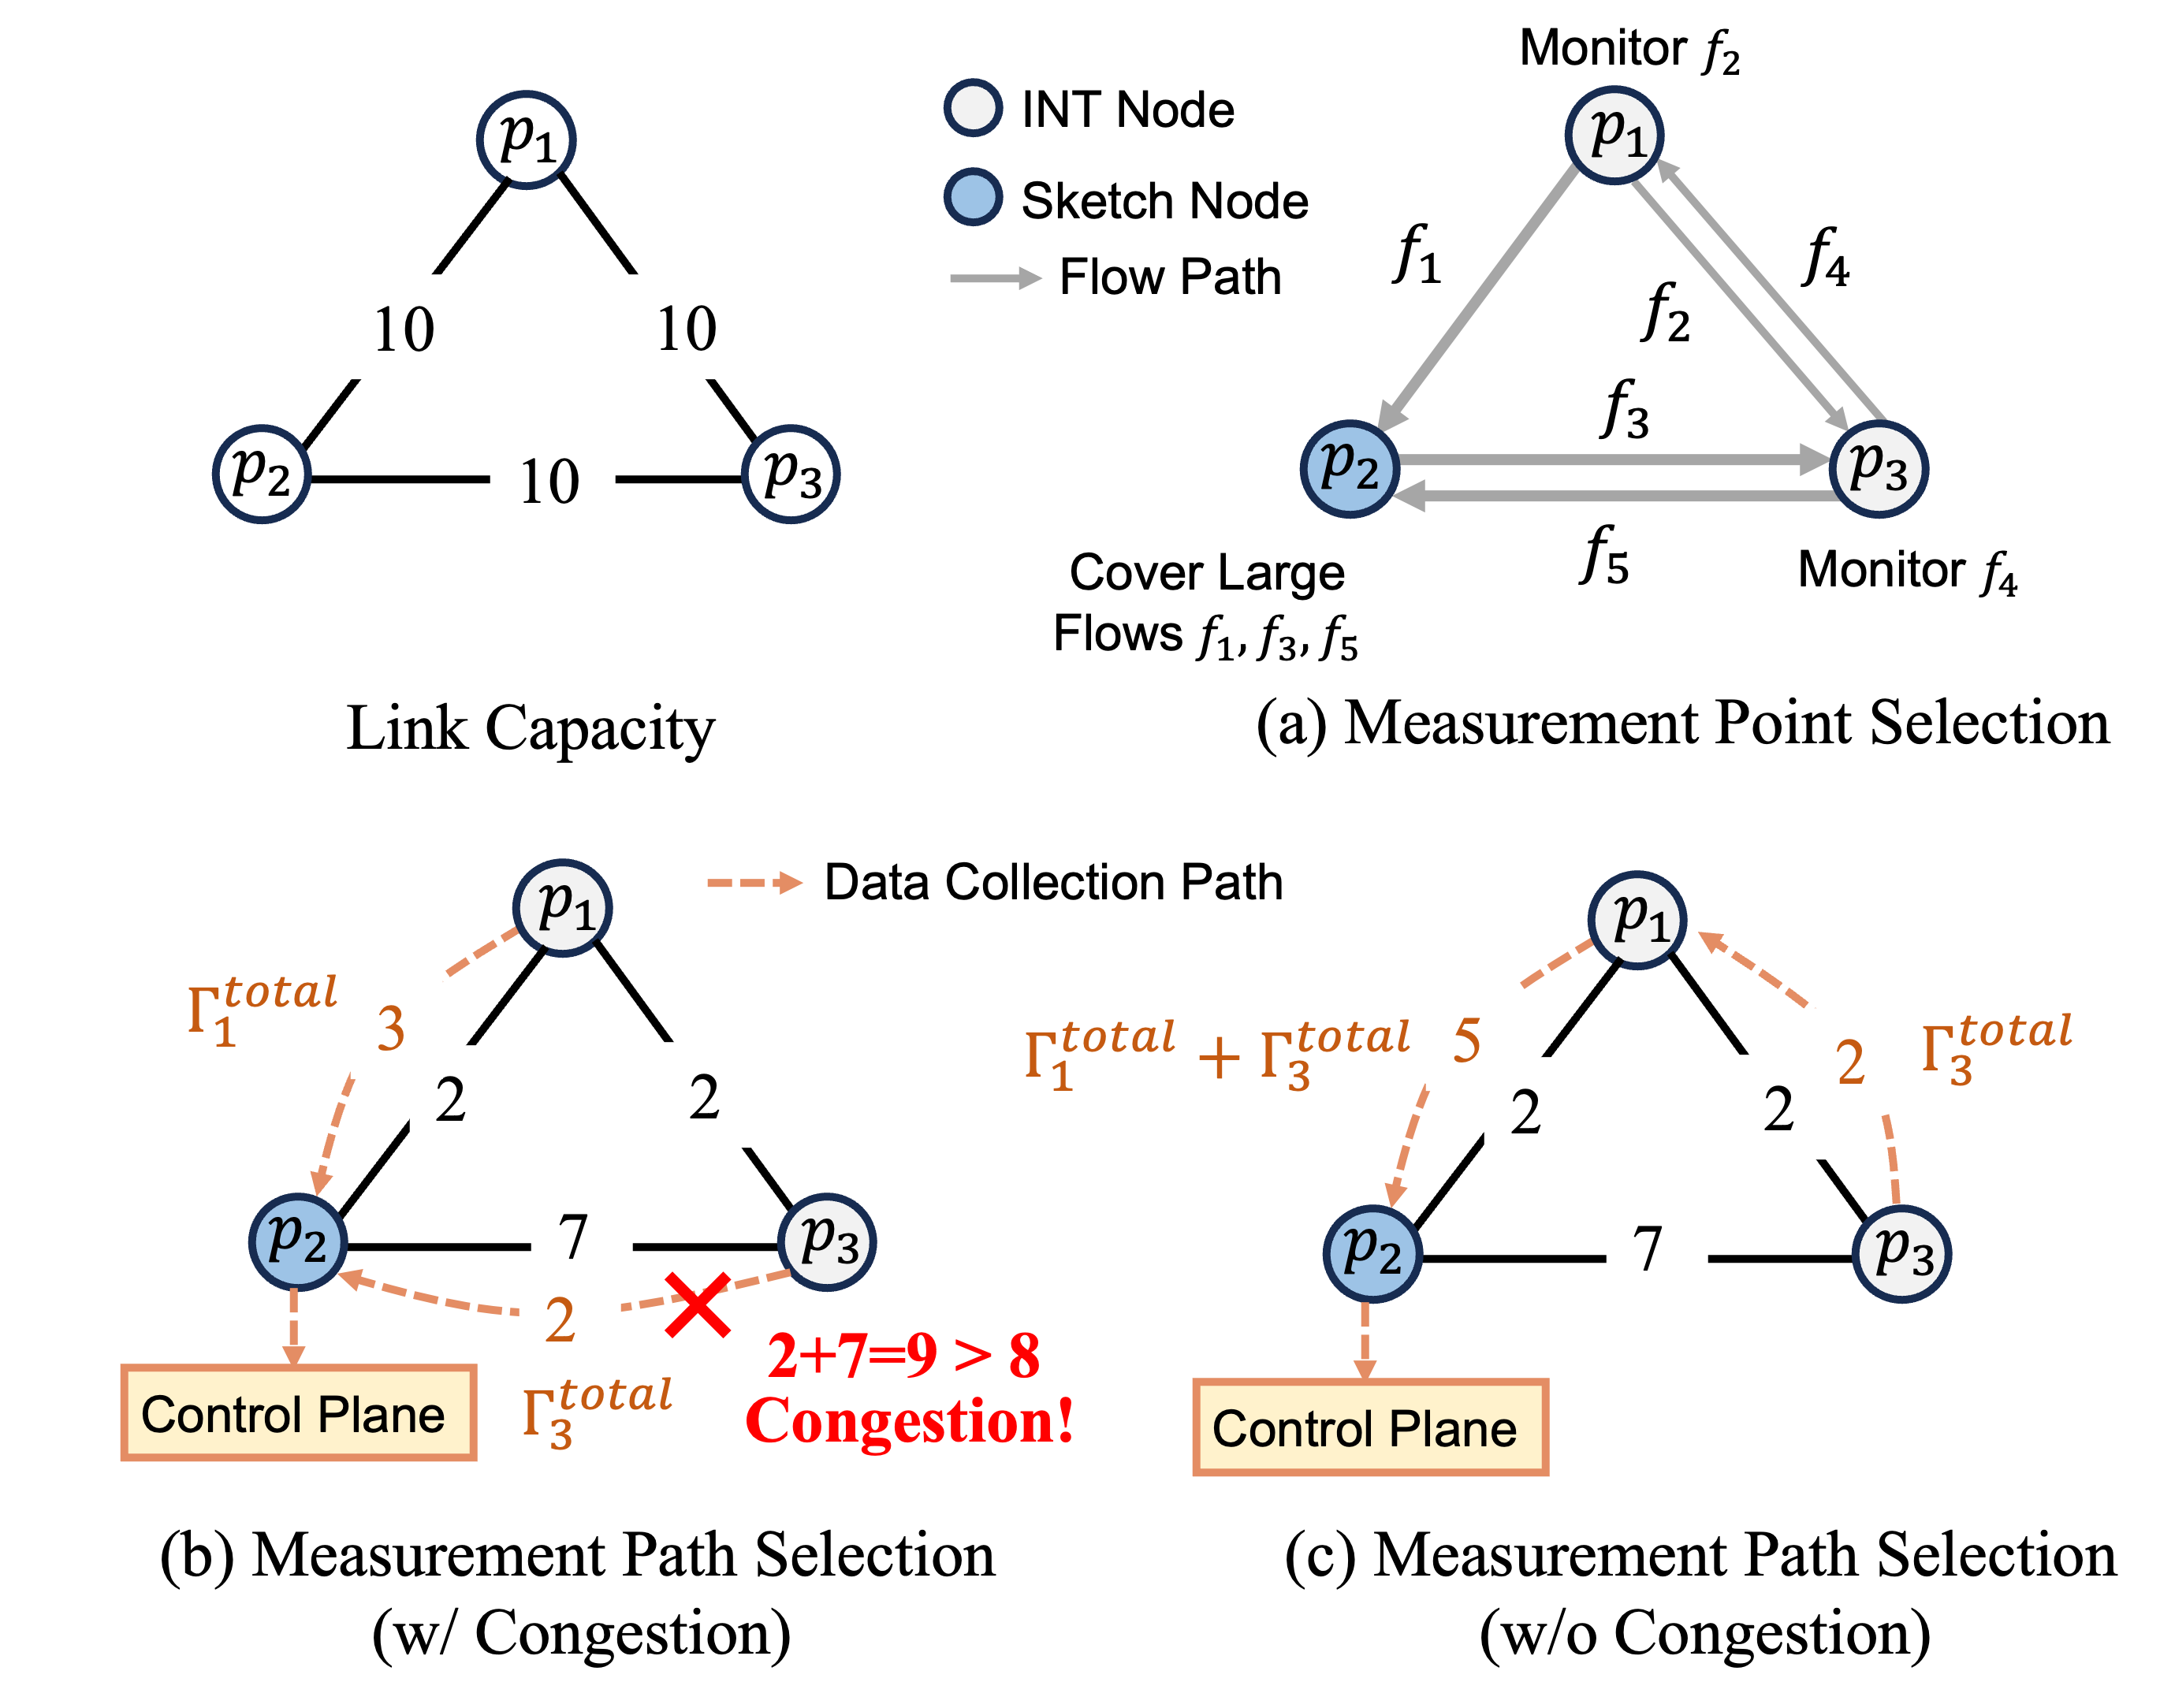
\includegraphics[width=\linewidth]{pics/example.png}
    \caption{Example of path selection in MonPlan.}
    \label{example}
\end{figure}

We present a simple example to explain how \sysname works. 

\para{Settings}. We consider a network comprising a triangle of three programmable switches, $p_1$, $p_2$, $p_3$. All links are 10-Gbps. The control plane is directly connected to $p_2$. Five flows traverse the network: a video flow $f_1$ with the OD pair of ($p_1$,$p_2$), a RPC flow $f_2$ with the OD pair of ($p_1$,$p_3$), a database flow $f_3$ with the OD pair of ($p_2$,$p_3$), an IoT flow $f_4$ with the OD pair of ($p_3$,$p_1$), and a backup flow $f_5$ with the OD pair of ($p_3$,$p_2$). $f_1$, $f_3$, and $f_5$ are large flows while small flows are $f_2$ and $f_4$. The safety threshold $\tau$ is 0.8 of link capacity. 

\para{Measurement point selection}. \sysname selects $p_2$ to deploy sketches. For large flows, $p_2$ covers all large flows, minimizing resource usage and data collection distance. For small flows, $p_1$ monitors $f_2$ while S3 monitors $f_4$. This decision achieves 100\% coverage while reducing the number of activated switches by 33\% compared to full INT deployment. 

%Thus, it balancing the tradeoff between coverage efficiency and proximity constraints through penalty weight optimization.

\para{Measurement data collection}. Consider the state $s_t$: (1) link utilizations: $p_1\leftrightarrow p_3=20$\%, $p_2\leftrightarrow p_3=70$\%, $p_1\leftrightarrow p_2=20$\%; (2) queue depths: 40\,KB in each switch; (3) worst-case measurement data rates: $\Gamma_{p_1}^{\text{total}}=3$\,Gbps, $\Gamma_{p_2}^{\text{total}}=1$\,Gbps, and $\Gamma_{p_3}^{\text{total}}=2$\,Gbps. The RL policy $\pi_{\theta}$ in \sysname decides to (1) deliver 100\% $p_1$'s INT data using the path $p_1\leftrightarrow p_2$, and (2) deliver 100\% $p_3$'s INT data using the path $p_3\rightarrow p_1\rightarrow p_2$. Otherwise, if $p_3$ sends INT data to $p_2$, the link $p_2\leftrightarrow p_3$ suffers from the load of 8\,Gbps, which violates the safety threshold $\tau$: $\Gamma_{p_3}^{\text{total}}+70$\%$\times 10$\,Gbps$=9$\,Gbps $> \tau\times 10$\,Gbps$=8$\,Gbps. This also avoids congesting other paths, e.g., for the path $p_1 \leftrightarrow p_2$, $\Gamma_{p_1}^{\text{total}}+\Gamma_{p_3}^{\text{total}}+20$\%$\times 10$\,Gbps$=7$\,Gbps $< \tau\times 10$\,Gbps$=8$\,Gbps, preserving the safety threshold and avoid data loss. 

% Queue depths: S1→S3=120 KB (congested), others=40 KB

% Worst-case rates: Γ<sub>S1</sub><sup>total</sup>=0.3 Gbps (INT for F2), Γ<sub>S3</sub><sup>total</sup>=0.15 Gbps (INT for F4)
% RL policy $\pi_θ$ outputs:

% Divert 70\% of S1's INT data through S1→S2→S3 (avoiding congested S1→S3)

% Route 100\% of S3's INT data via S3→S2 (direct path underutilized)
% Congestion safeguard scales ratios to ensure:

% S1→S2: 60\% + (0.3×0.7×10\%)=62.1\% < 80\%

% S3→S2: 82% + 1.5%=83.5% → over threshold! → dynamically reroutes 30% to S3→S1→S2
% Final deployment achieves zero packet loss with 43 μs INT latency.

%Consider that the current link utilizations: S1$\rightarrow$S2=65\%, S2$\rightarrow$S3=72\%, S3$\rightarrow$S2=60\%; queue depths are 50\,KB; and the worst-case measurement data rates: 0.5\,Gbps from S1, 7\,Gbps from S2, and 0.3\,Gbps from S3. The decisions of \sysname are: 100\% of S1's INT data (measuring $f_2$) and S3's INT data (measuring $f_4$) are transferred through the path S1$\rightarrow$S2 and the path S3$\rightarrow$S2, respectively. Therefore, none of links will exceed the safety threshold.  

%The RL policy processes real-time telemetry (link utilizations: S1→S2=65\%, S2→S3=72\%, S3→S2=60\%; queue depths: 50\,KB uniform) and worst-case measurement rates (S1:0.5Gbps, S2:7Gbps, S3:0.3Gbps). It outputs direct-path routing: 100\% of S1's INT data (F2) and S3's INT data (F4) through S1→S2 and S3→S2 respectively. The congestion safeguard validates projected utilization (S1→S2: 65\% + 5\% = 70\% $<$ 80\% threshold; S3→S2: 60\% + 3\% = 63\% $<$ 80\%), confirming loss-free transmission without scaling. P4 flow rules enforce these paths dynamically during traffic spikes.




